\documentclass[a4paper,14pt]{article}

%%% Работа с русским языком
\usepackage{cmap}					% поиск в PDF
\usepackage{mathtext} 				% русские буквы в формулах
\usepackage[T2A]{fontenc}			% кодировка
\usepackage[utf8]{inputenc}			% кодировка исходного текста
\usepackage[english,russian]{babel}	% локализация и переносы
\usepackage{indentfirst}
\frenchspacing

\newcommand{\vyp}{\ensuremath{\hookrightarrow}}
\renewcommand{\epsilon}{\ensuremath{\varepsilon}}
\renewcommand{\phi}{\ensuremath{\varphi}}
\renewcommand{\kappa}{\ensuremath{\varkappa}}
\renewcommand{\le}{\ensuremath{\leqslant}}
\renewcommand{\leq}{\ensuremath{\leqslant}}
\renewcommand{\ge}{\ensuremath{\geqslant}}
\renewcommand{\geq}{\ensuremath{\geqslant}}
\renewcommand{\emptyset}{\varnothing}
\newcommand{\Ra}{\ensuremath{\Rightarrow}}
\newcommand{\ra}{\ensuremath{\rightarrow}}
\newcommand{\LRa}{\ensuremath{\Leftrightarrow}}
\newcommand{\tbf}{\textbf}
\newcommand{\ov}{\ensuremath{\overline}}
\newcommand{\CC}{\ensuremath{\mathbb{C}}}
\newcommand{\RR}{\ensuremath{\mathbb{R}}}
\newcommand{\NN}{\ensuremath{\mathbb{N}}}
\newcommand{\QQ}{\ensuremath{\mathbb{Q}}}
\newcommand{\ZZ}{\ensuremath{\mathbb{Z}}}

%%% Дополнительная работа с математикой
\usepackage{amsmath,amsfonts,amssymb,amsthm,mathtools} % AMS
\usepackage{icomma} % "Умная" запятая: $0,2$ --- число, $0, 2$ --- перечисление

%% Номера формул
%\mathtoolsset{showonlyrefs=true} % Показывать номера только у тех формул, на которые есть \eqref{} в тексте.
%\usepackage{leqno} % Нумереация формул слева

%% Свои команды
\DeclareMathOperator{\sgn}{\mathop{sgn}}

%% Перенос знаков в формулах (по Львовскому)
\newcommand*{\hm}[1]{#1\nobreak\discretionary{}
{\hbox{$\mathsurround=0pt #1$}}{}}



%%% Работа с картинками
\usepackage{graphicx}  % Для вставки рисунков
\graphicspath{{images/}{images2/}}  % папки с картинками
\setlength\fboxsep{3pt} % Отступ рамки \fbox{} от рисунка
\setlength\fboxrule{1pt} % Толщина линий рамки \fbox{}
\usepackage{wrapfig} % Обтекание рисунков текстом

%%% Работа с таблицами
\usepackage{array,tabularx,tabulary,booktabs} % Дополнительная работа с таблицами
\usepackage{longtable}  % Длинные таблицы
\usepackage{multirow} % Слияние строк в таблице

%%% Теоремы
\theoremstyle{plain} % Это стиль по умолчанию, его можно не переопределять.
\newtheorem{theorem}{Теорема}[section]
\newtheorem{proposition}[theorem]{Утверждение}
 
\theoremstyle{definition} % "Определение"
\newtheorem{corollary}{Следствие}[theorem]
\newtheorem{problem}{Задача}[section]
 
\theoremstyle{remark} % "Примечание"
\newtheorem*{nonum}{Решение}

%%% Программирование
\usepackage{etoolbox} % логические операторы

%%% Страница
\usepackage{extsizes} % Возможность сделать 14-й шрифт
\usepackage{geometry} % Простой способ задавать поля
	\geometry{top=20mm}
	\geometry{bottom=20mm}
	\geometry{left=5mm}
	\geometry{right=15mm}
 %
\usepackage{fancyhdr} % Колонтитулы
 	\pagestyle{fancy}
 	\renewcommand{\headrulewidth}{1pt}  % Толщина линейки, отчеркивающей верхний колонтитул
%\fancypagestyle{firstpage}{
	\rhead{\large{Исыпов Илья}}
%}
% 	\lfoot{Нижний левый}
% 	\rfoot{\large{Рябых Владислав, Б05-905}}
% 	\rhead{Верхний правый]}
% 	\chead{Верхний в центре}
 	\lhead{\large{Рябых Владислав}}
%	\cfoot{Нижний в центре} % По умолчанию здесь номер страницы

\usepackage{setspace} % Интерлиньяж
\onehalfspacing % Интерлиньяж 1.5
%\doublespacing % Интерлиньяж 2
%\singlespacing % Интерлиньяж 1

\usepackage{lastpage} % Узнать, сколько всего страниц в документе.

\usepackage{soul} % Модификаторы начертания

\usepackage{hyperref}
\usepackage[usenames,dvipsnames,svgnames,table,rgb]{xcolor}
\hypersetup{				% Гиперссылки
    unicode=true,           % русские буквы в раздела PDF
    pdftitle={Заголовок},   % Заголовок
    pdfauthor={Автор},      % Автор
    pdfsubject={Тема},      % Тема
    pdfcreator={Создатель}, % Создатель
    pdfproducer={Производитель}, % Производитель
    pdfkeywords={keyword1} {key2} {key3}, % Ключевые слова
    colorlinks=true,       	% false: ссылки в рамках; true: цветные ссылки
    linkcolor=red,          % внутренние ссылки
    citecolor=black,        % на библиографию
    filecolor=magenta,      % на файлы
    urlcolor=cyan           % на URL
}

\usepackage{csquotes} % Еще инструменты для ссылок

%\usepackage[style=authoryear,maxcitenames=2,backend=biber,sorting=nty]{biblatex}

\usepackage{multicol} % Несколько колонок

\usepackage{tikz} % Работа с графикой
\usepackage{pgfplots}
\usepackage{pgfplotstable}

\usepackage{caption}
\long\def\comment{}
\setlength{\abovecaptionskip}{7pt}
\setlength{\belowcaptionskip}{7pt}


\begin{document}
\author{Рябых Владислав и Валеев Сергей, Б05-905}
\title{\tbf{3.6.1. Спектральный анализ электрических сигналов}}
\maketitle

\tbf{Цель работы:} изучение спектрального состава периодических электрических сигналов.

\tbf{В работе используются:} персональный компьютер, USB-осциллограф АКИП-4107,  функциональный генератор WaveStation 2012, соединительные кабели.


\section*{Теория}

В работе изучается спектральный состав периодических электрических сигналов различной формы: последовательности прямоугольных импульсов, последовательности цугов и амплитудно-модулированных гармонических колебаний. Спектры этих сигналов наблюдаются с помощью промышленного анализатора спектра и сравниваются с рассчитанными теоретически. 

Функциональный генератор WaveStation 2012 позволяет сформировать два различных электрических сигнала, которые выводятся на два независимых канала -- CH1 и CH2. Сигнал с первого канала подается на вход A, а сигнал со второго канала на вход B USB-осциллографа. Затем эти сигналы подаются на вход компьютера через USB-соединение. При работе USB-осциллографа в режиме осциллографа, на экране компьютера можно наблюдать каждый из сигналов в отдельности, а также их произведение. В режиме спектроанализа можно наблюдать спектры этих сигналов.

\begin{figure}[!h]
	\centering
	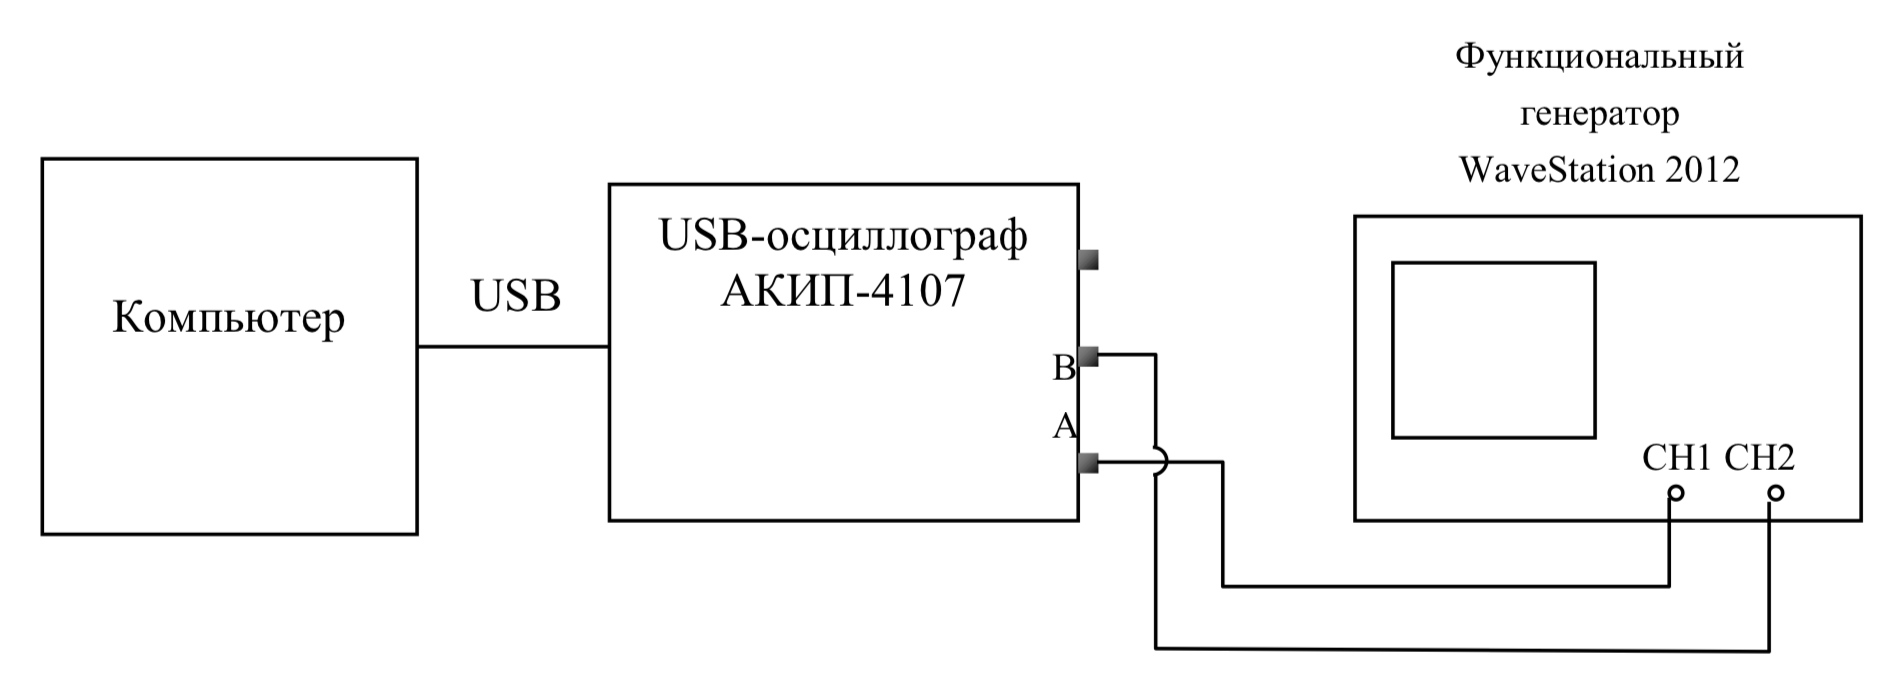
\includegraphics[width = 12cm]{first} \\
	Рис. 1 -- Структурная схема анализатора спектра
\end{figure}

\section*{Ход работы}

\subsection*{Исследование спектра периодической последовательности\\ прямоугольных импульсов}

Проведём анализ спектра периодической последовательности прямоугольных импульсов при различных значениях частоты повторения импульсов и длительности импульсов. Спектры полученные в ходе работы приведены на рисунках 2 -- 5.
Проведем измерения зависимости ширины спектра $\Delta \nu$ от длительности импульса $\tau$, результаты измерений запишем в таблицу \ref{tab1}.

\begin{table}[hbt!]
	\begin{center}
	\begin{tabular}{|c|c|c|c|c|c|c|c|c|}
		\hline
		$\Delta \nu$, кГц                & 25 & 16.3 & 12.5 & 8.72 & 7   & 6.2 & 5.6 & 5   \\ \hline
		$\tau$, мкс                      & 40 & 60   & 80   & 120  & 140 & 160 & 180 & 200 \\ \hline
		1/$\tau$, $10^3 \cdot \text{с}^{-1}$ & 25 & 16.7 & 12.5 & 8.3  & 7.1 & 6.3 & 5.6 & 5   \\ \hline
	\end{tabular}
\caption{результаты измерений}
\label{tab1}
\end{center}
\end{table}

\begin{figure}[!h]
	\parbox[!h]{0.5\textwidth}{\null
		\centering
		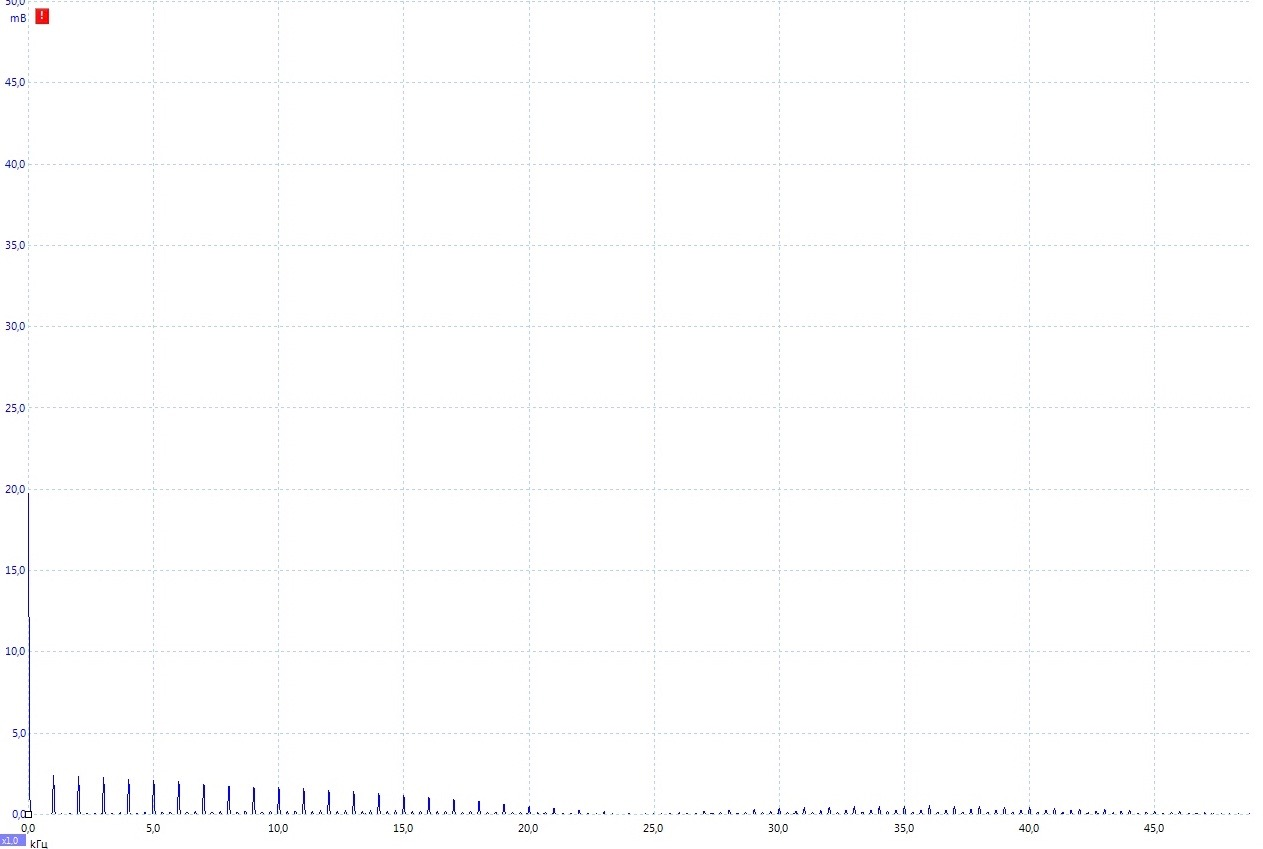
\includegraphics[width = 9cm]{2.jpeg}
		Рис. 2 -- $f_{\text{повт}} = 1$ кГц, $\tau = 50$ мкс}
	\parbox[!h]{0.5\textwidth}{\null
		\centering
		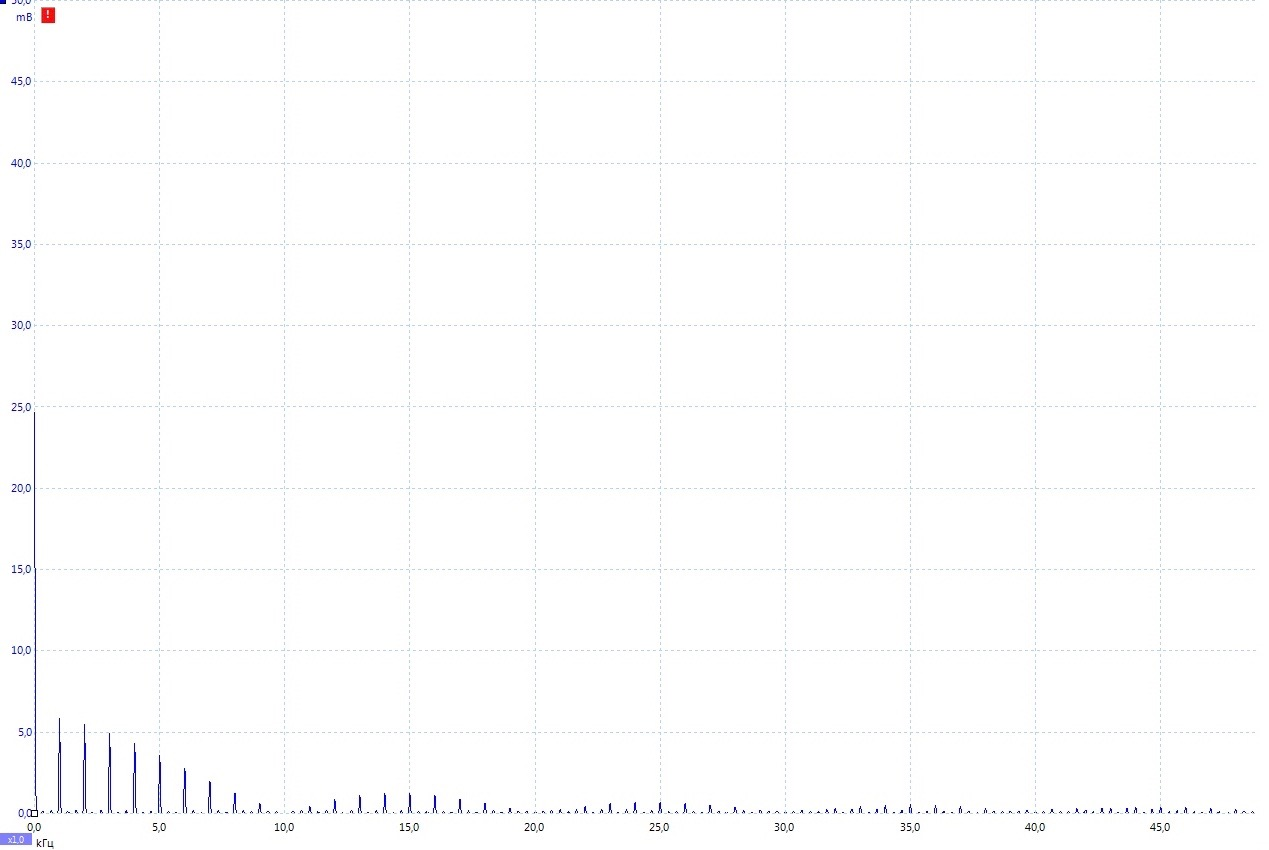
\includegraphics[width = 9cm]{3.jpeg} \\
		Рис. 3 -- $f_{\text{повт}} = 1$ кГц, $\tau = 100$ мкс}
\end{figure}

\begin{figure}[!h]
\parbox[!h]{0.5\textwidth}{\null
	\centering
	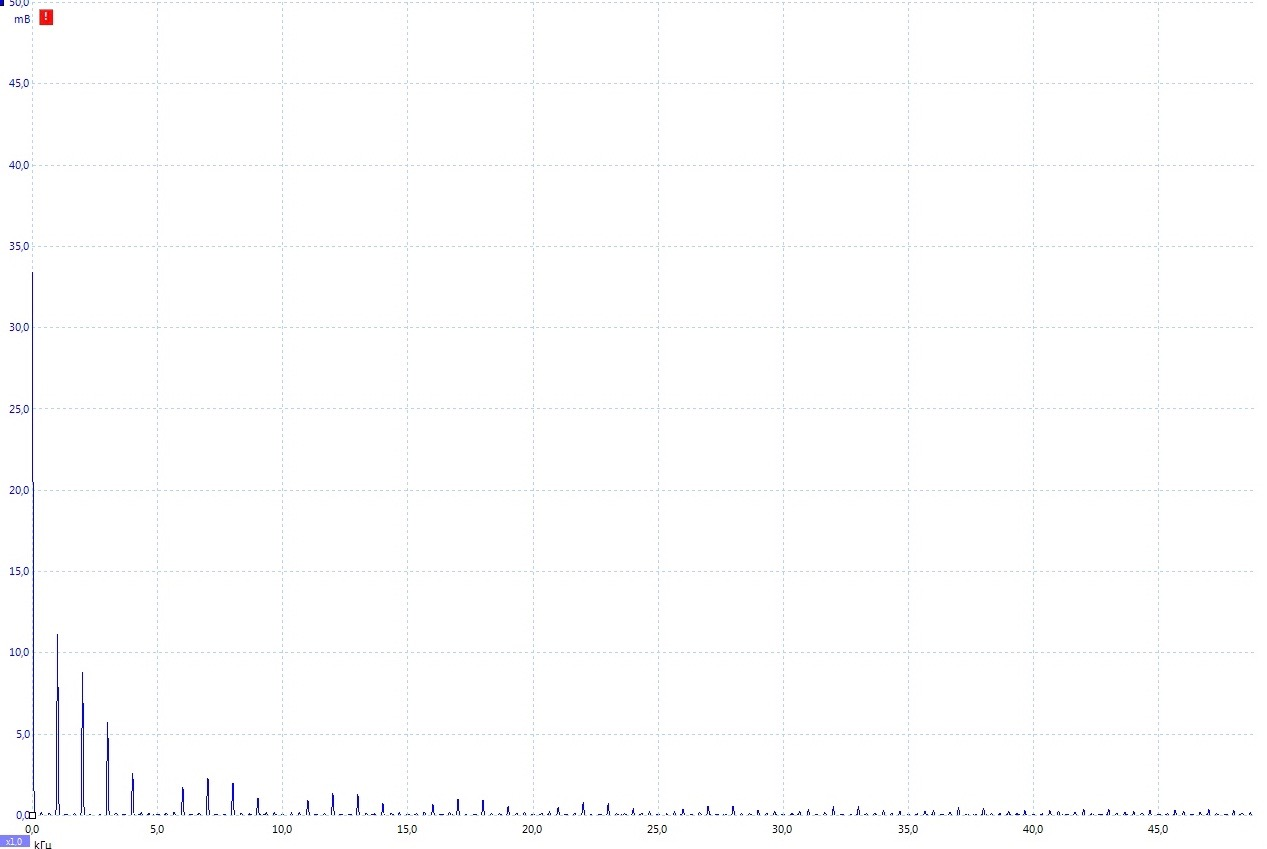
\includegraphics[width = 9cm]{4.jpeg}
	Рис. 4 -- $f_{\text{повт}} = 2$ кГц, $\tau = 100$ мкс}
\parbox[!h]{0.5\textwidth}{\null
	\centering
	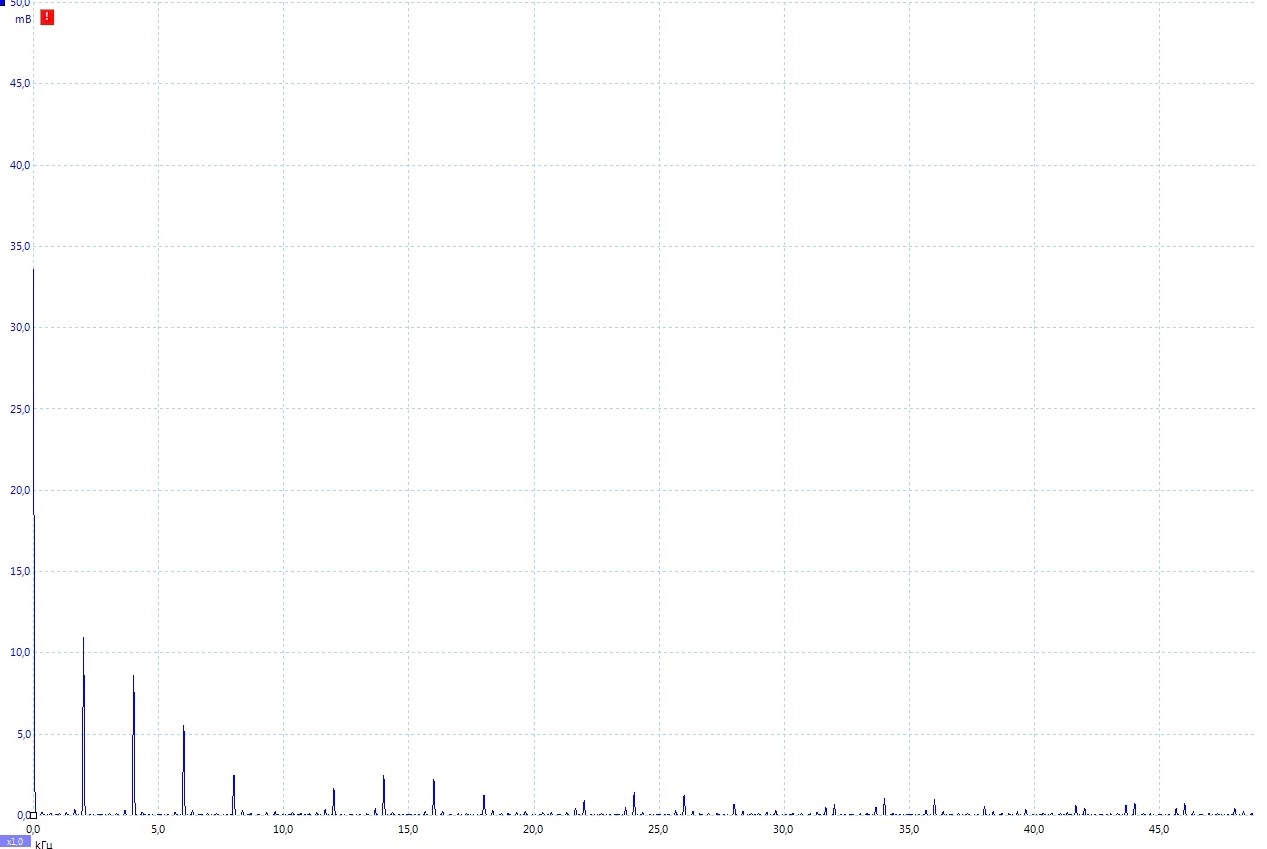
\includegraphics[width = 9cm]{5.jpeg} \\
	Рис. 5 -- $f_{\text{повт}} = 1$ кГц, $\tau = 50$ мкс}
\end{figure}

При частоте повторения сигналов $f_\text{повт} = 1$ кГц  и $\tau = 50$ мкс измерим частоты и амплитуды спектральных составляющих сигнала и запишем результаты в таблице \ref{tab2}. Аналогичные измерения проведем при $\tau = 100$ мкс, результаты см. в таблице \ref{tab3}. 


\begin{table}[hbt!]
\begin{center}
\begin{tabular}{|c|c|c|c|c|c|c|c|c|c|c|c|}
	\hline
	№ гармоники & 0     & 1     & 2     & 3     & 4     & 5     & 6     & 7     & 8     & 9     & 10    \\ \hline
	$\nu$, кГц      & 0.01  & 1.002 & 1.999 & 2.981 & 4.008 & 5.001 & 5.998 & 7.006 & 8.012 & 8.989 & 10    \\ \hline
	$A$, мВ         & 141.5 & 69.32 & 68.7  & 65.87 & 62.74 & 58.66 & 56.78 & 52.07 & 47.68 & 43.91 & 40.78 \\ \hline
\end{tabular}
\caption{результаты измерений при $f_\text{повт} = 1$ кГц  и $\tau = 50$ мкс}
\label{tab2}
\end{center}
\end{table}

\begin{table}[hbt!]
	\begin{center}
		\begin{tabular}{|c|c|c|c|c|c|c|c|c|c|c|c|}
			\hline
			№ гармоники & 0     & 1     & 2     & 3     & 4     & 5     & 6     & 7     & 8     & 9     & 10 \\ \hline
			$\nu$, кГц      & 0.005 & 1.007 & 1.999 & 3.006 & 4.003 & 5.01  & 6.012 & 6.999 & 7.961 & 9.011 & --  \\ \hline
			$A$, мВ         & 243.4 & 136.1 & 128.6 & 117.9 & 103.8 & 85.95 & 68.07 & 48.31 & 32.94 & 14.43 & --  \\ \hline
		\end{tabular}
		\caption{результаты измерений при $f_\text{повт} = 1$ кГц  и $\tau = 100$ мкс}
		\label{tab3}
	\end{center}
\end{table}

По результатам измерений построим график зависимости $\Delta \nu = f(1/\tau)$, см. на рис. 6. Убеждаемся в справедливости соотношения неопределенностей: коэффициент наклона графика $k \approx 1$.


\begin{center}
	\begin{figure}[hbt!]
		\centering
		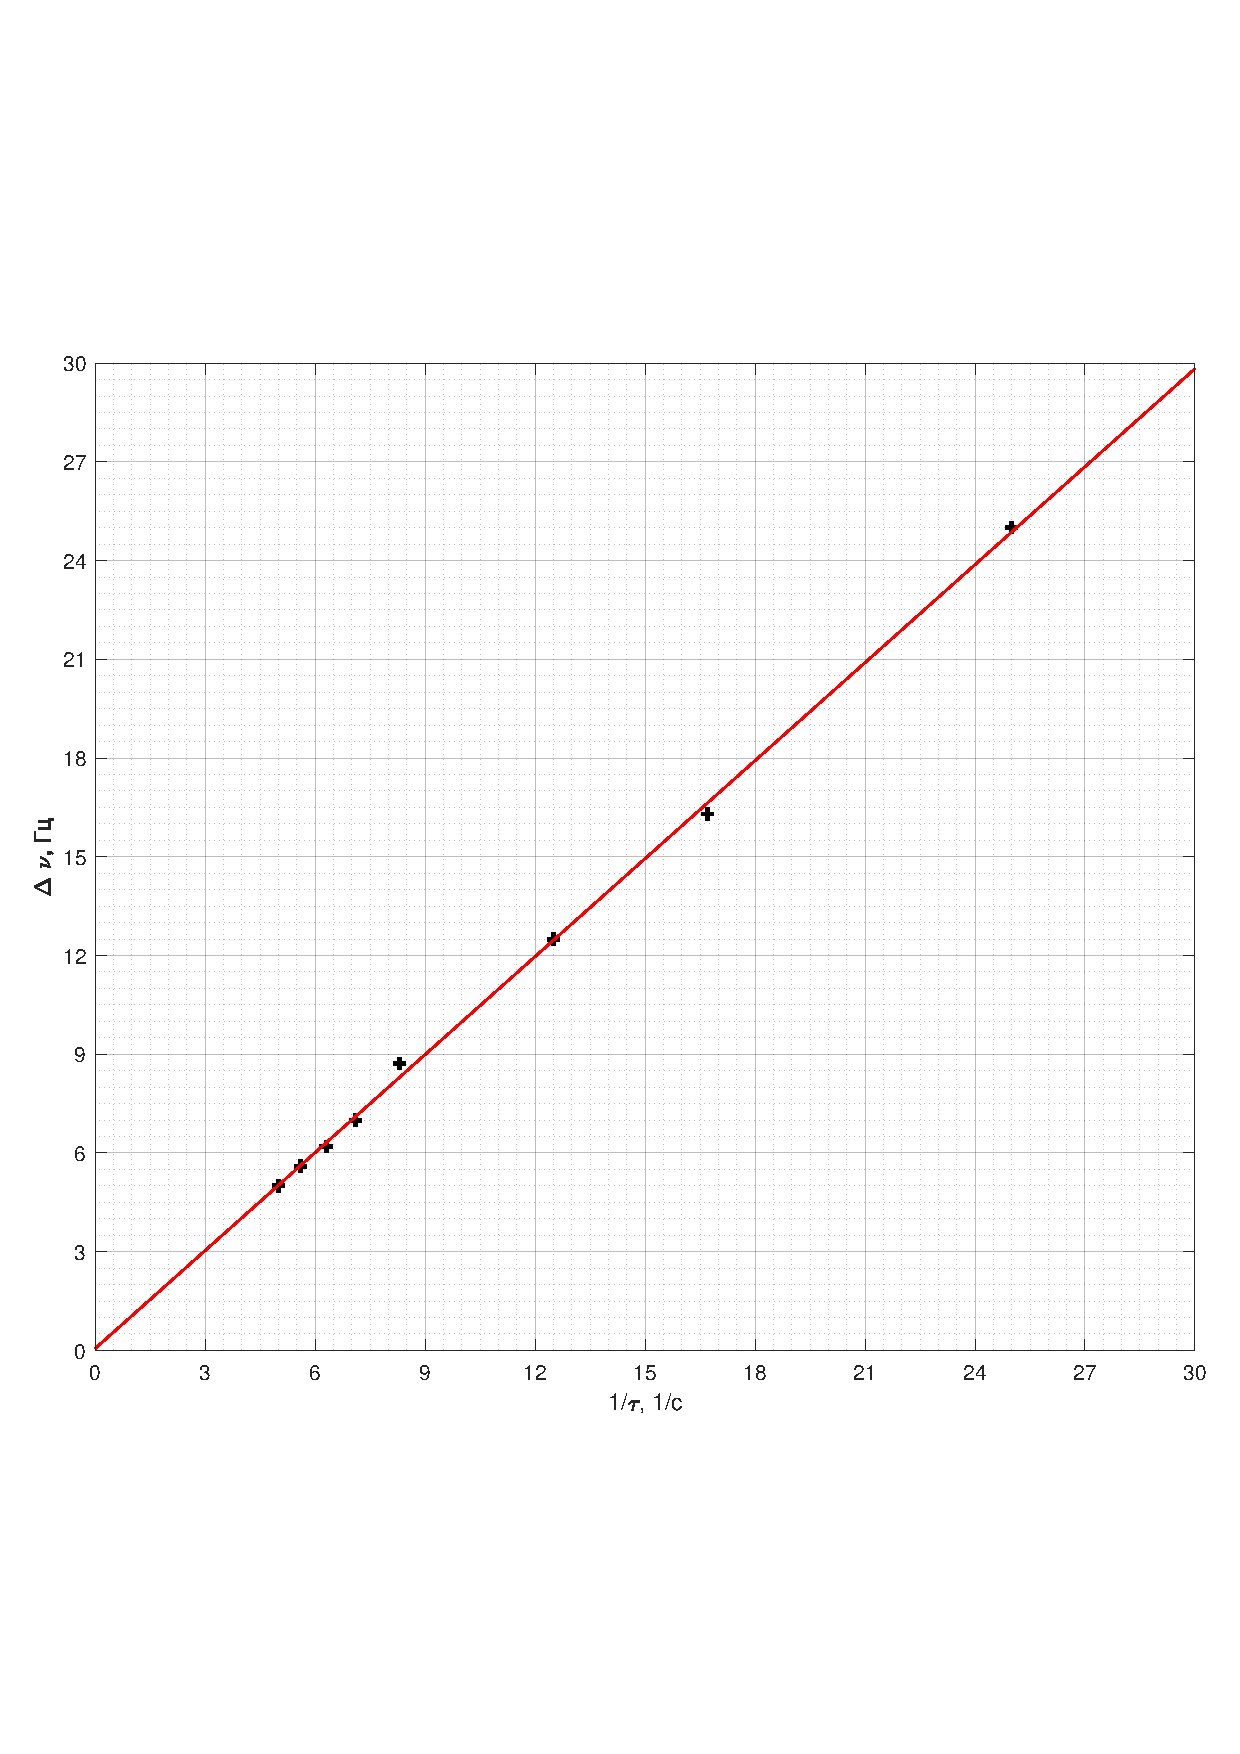
\includegraphics[width=0.7\linewidth]{gr1.pdf} \\
		Рис. 6 -- График зависимости $\Delta \nu(1/\tau)$
		\label{gr1}
	\end{figure}
\end{center}

\subsection*{Исследование спектра периодической последовательности цугов гармонических колебаний}

Установим частоту несущей $\nu_0 = 25$ кГц, проведем анализ спектра при различных параметрах сигнала. Спектры при различных параметрах см. на рис. 7 -- 10.

\begin{figure}[!h]
	\parbox[!h]{0.5\textwidth}{\null
		\centering
		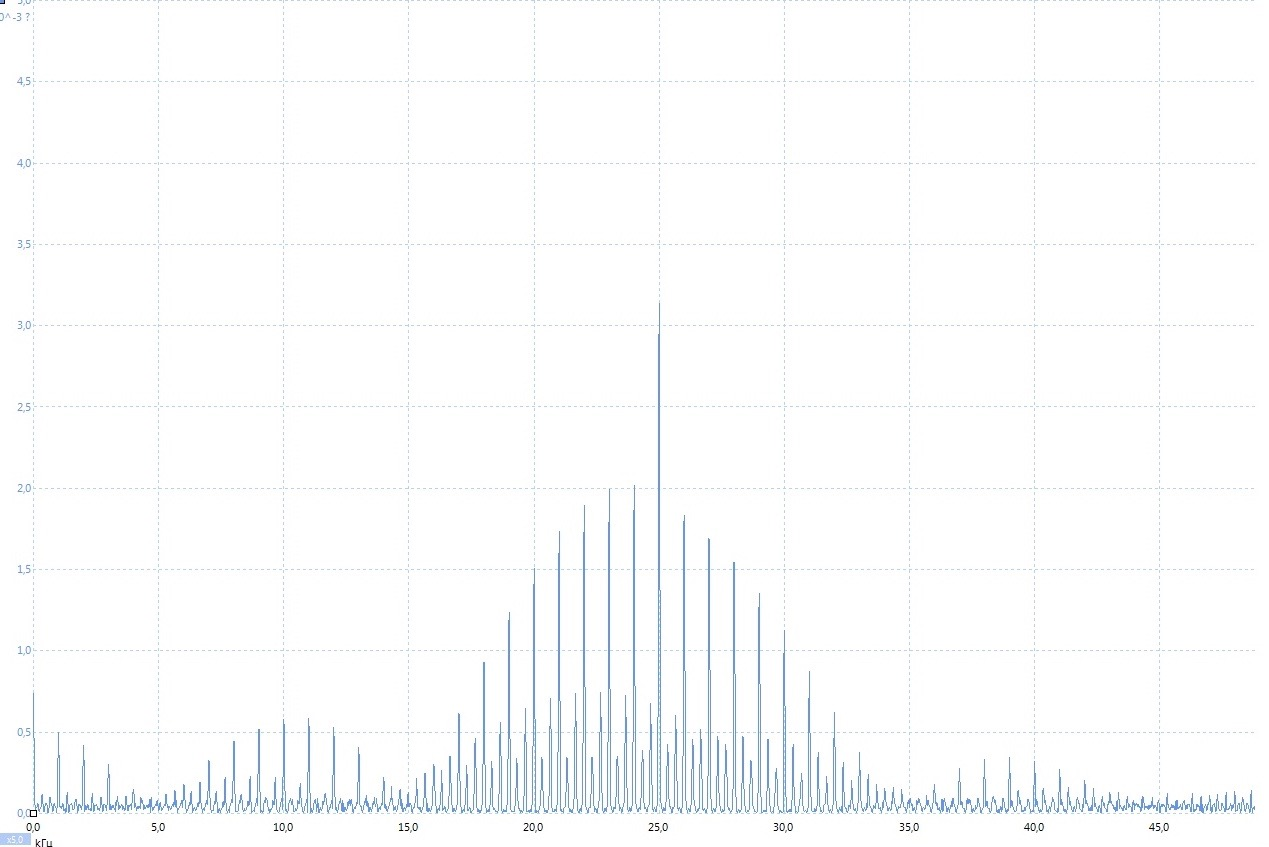
\includegraphics[width = 9cm]{6.jpeg}
		Рис. 7 -- Спектр при $f_{\text{повт}} = 1$ кГц, $\tau = 100$ мкс, $\nu_0 =25$ кГц}
	\parbox[!h]{0.5\textwidth}{\null
		\centering
		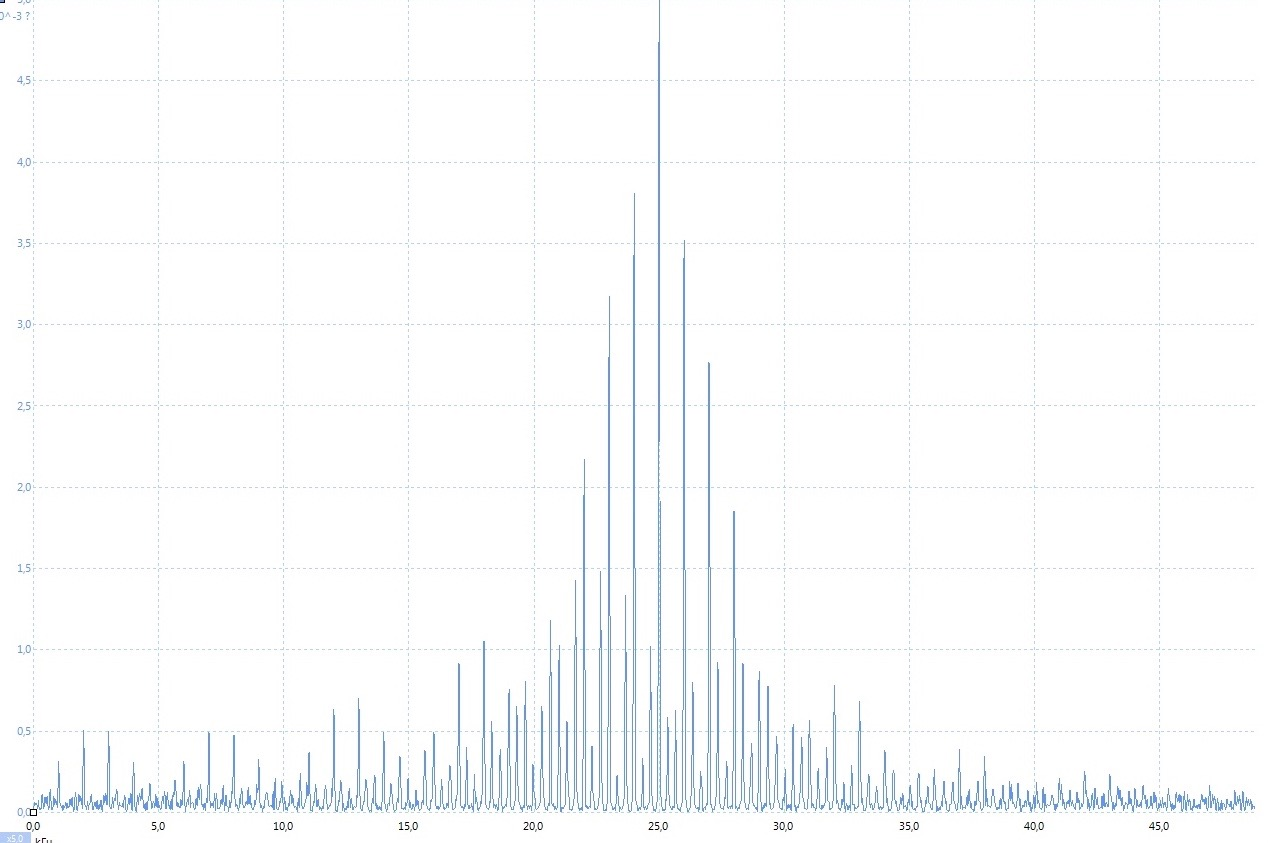
\includegraphics[width = 9cm]{7.jpeg} \\
		Рис. 8 -- Спектр при $f_{\text{повт}} = 1$ кГц, $\tau = 200$ мкс, $\nu_0 = 25$ кГц}
	\parbox[!h]{0.5\textwidth}{\null
		\centering
		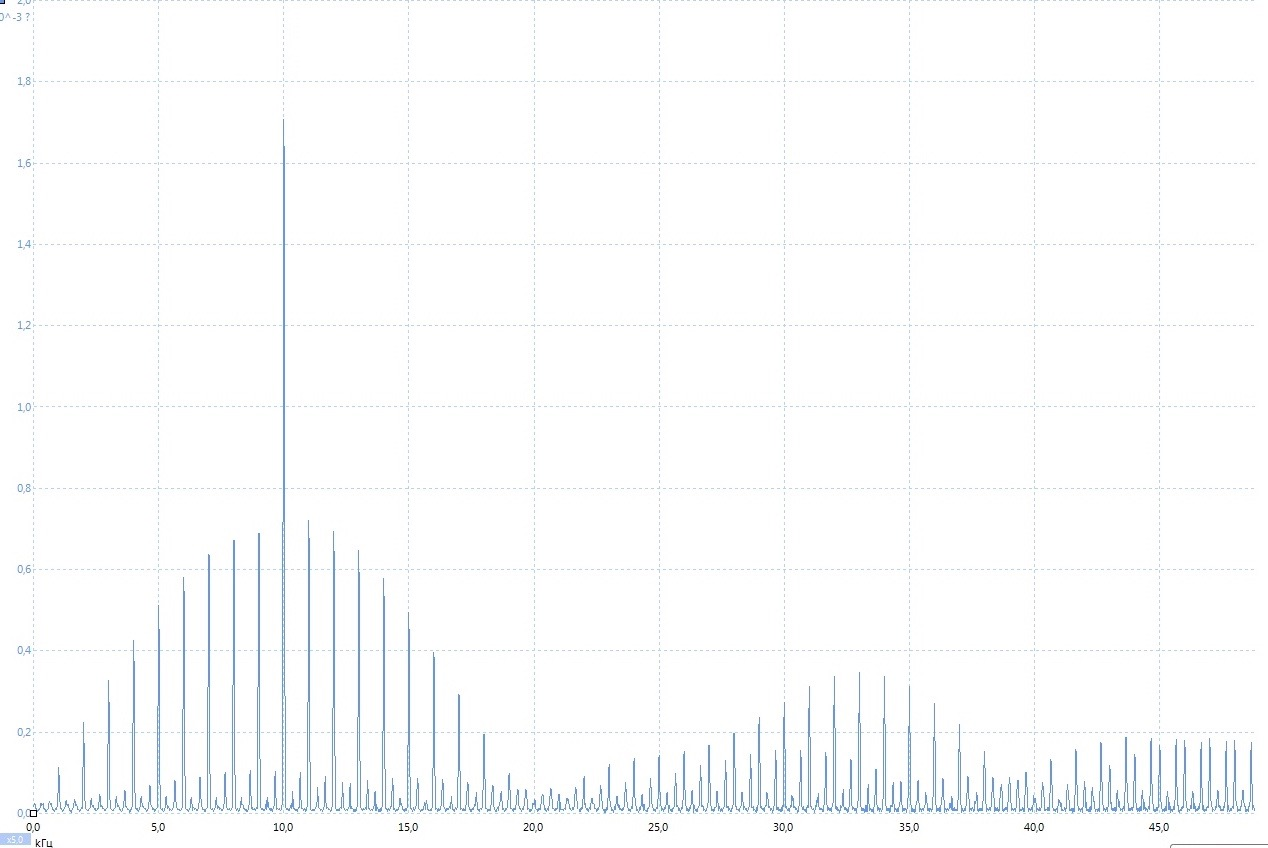
\includegraphics[width = 9cm]{8.jpeg}
		Рис. 9 -- Спектр при $f_{\text{повт}} = 1$ кГц, $\tau = 100$ мкс, $\nu_0 = 10$ кГц}
	\parbox[!h]{0.5\textwidth}{\null
		\centering
		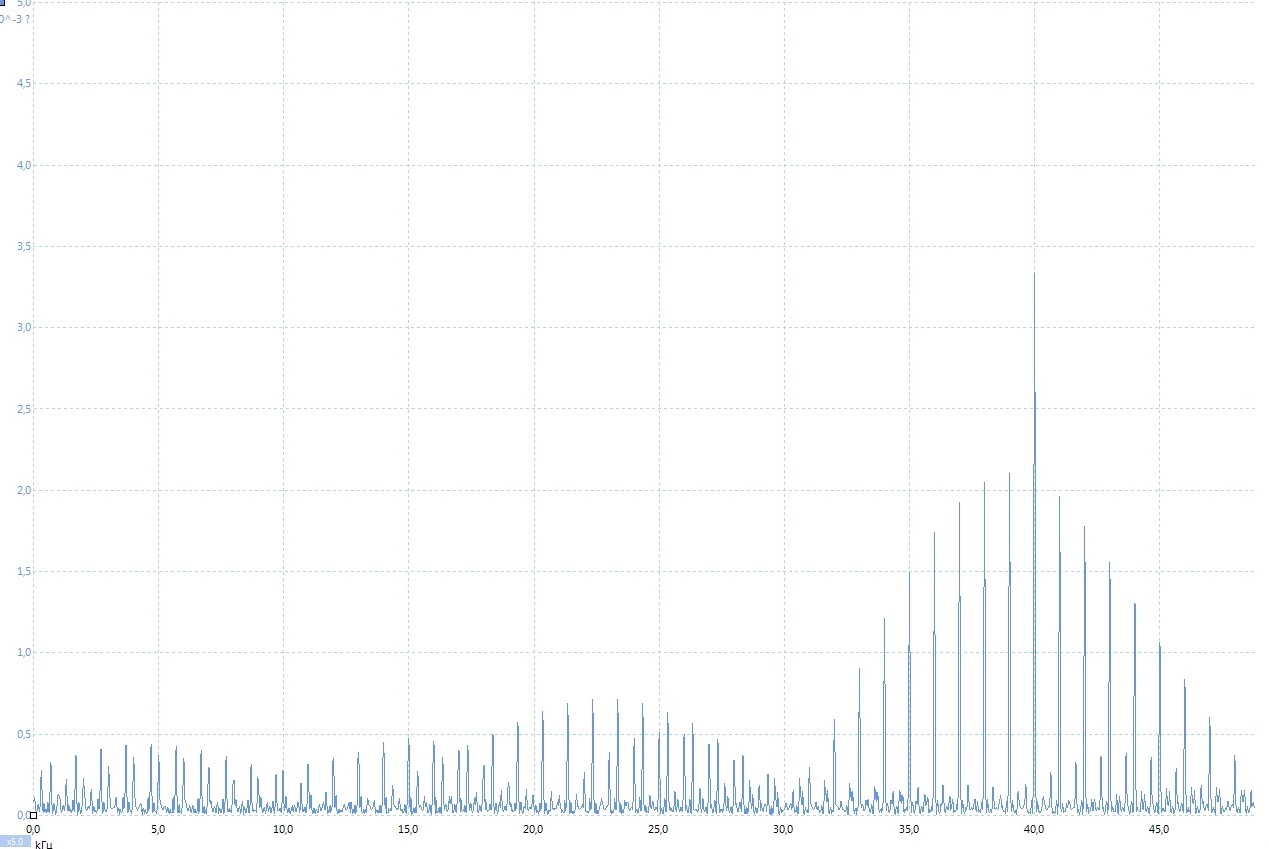
\includegraphics[width = 9cm]{10.jpeg} \\
		Рис. 10 -- Спектр при $f_{\text{повт}} = 1$ кГц, $\tau = 100$ мкс, $\nu_0 = 40$ кГц}
\end{figure}


Проведем измерения зависимости ширины спектра $\Delta \nu$ от частоты повторения импульсов $f_{\text{повт}}$, результаты измерений запишем в таблицу \ref{tab4}.

\begin{table}[hbt!]
	\begin{center}
	\begin{tabular}{|c|c|c|c|c|c|} \hline
		$\Delta \nu$, кГц	& 1.00 & 2.00 & 3.00 & 4.00 & 5.00\\ \hline
		$f_{\text{повт}}$, кГц & 1.00 & 2.00 & 3.00 & 4.00 & 5.00 \\ \hline
	\end{tabular}
\caption{результаты измерений}
\label{tab4}
\end{center}
\end{table}

При частоте повторения сигналов $f_\text{повт} = 1$ кГц  и $\tau = 100$ мкс измерим частоты и амплитуды спектральных составляющих сигнала и запишем результаты в таблицу \ref{tab5}. Аналогичные измерения проведем при $f_\text{повт} = 2$ кГц, результаты см. в таблице \ref{tab6}. 

\begin{table}[hbt!]
	\begin{center}
	\begin{tabular}{|c|c|c|c|c|c|c|c|c|c|c|c|c|c|c|c|c|c|} \hline
		$N_{\text{г}}$ &1&	2&	3&4&	5&	6&	7&8&	9&	10&	11&	12	&13	&14&	15	&16&	17\\ \hline
		$\nu$, кГц	&20	&21&	22&	23&	24&	25&	26&	27&	28&	29&	30&	31&	32&	33&	34&	35&	36\\ \hline
		$A, \text{мкВ}$&	0	&1.7&	3.7&	5.9&	7.7&	9.2&	10&	11.6&	12.6	&13&	15.6&	14&	13&	12&	10.7&	9&	6.8	 \\ \hline
	\end{tabular}
	\caption{Результаты измерений при $f_\text{повт} = 1$ кГц  и $\tau = 100$ мкс}
	\label{tab5}
\end{center}
\end{table}


%$N_{\text{г}}$&
%$\nu$, кГц	&
%$A, \text{мкВ}$&

\begin{table}[hbt!]
	\begin{center}
	\begin{tabular}{|c|c|c|c|c|c|c|c|c|c|c|} \hline
		$N_{\text{г}}$&1&	2&	3&4&	5&	6&	7&8&	9 & 	10\\ \hline
		$\nu$, кГц	&20&	22&	24	&26	&28&	30&	32&	34&	36&	38 \\ \hline
			$A, \text{мкВ}$&0	&7.50&	15.4&	21.3&	25.7&	29.3&	26.2&	21.0&	13.8&	6.2\\ \hline
	\end{tabular}
\caption{Результаты измерений при $f_\text{повт} = 2$ кГц  и $\tau = 100$ мкс}
\label{tab6}
\end{center}
\end{table}

По результатам измерений построим график зависимости $\Delta \nu(f_{\text{повт}})$, и убедимся в справедливости соотношения неопределенностей, так как наклон графика $k \approx 1$, см. на рис. 11.

\begin{center}
	\begin{figure}[hbt!]
		\centering
		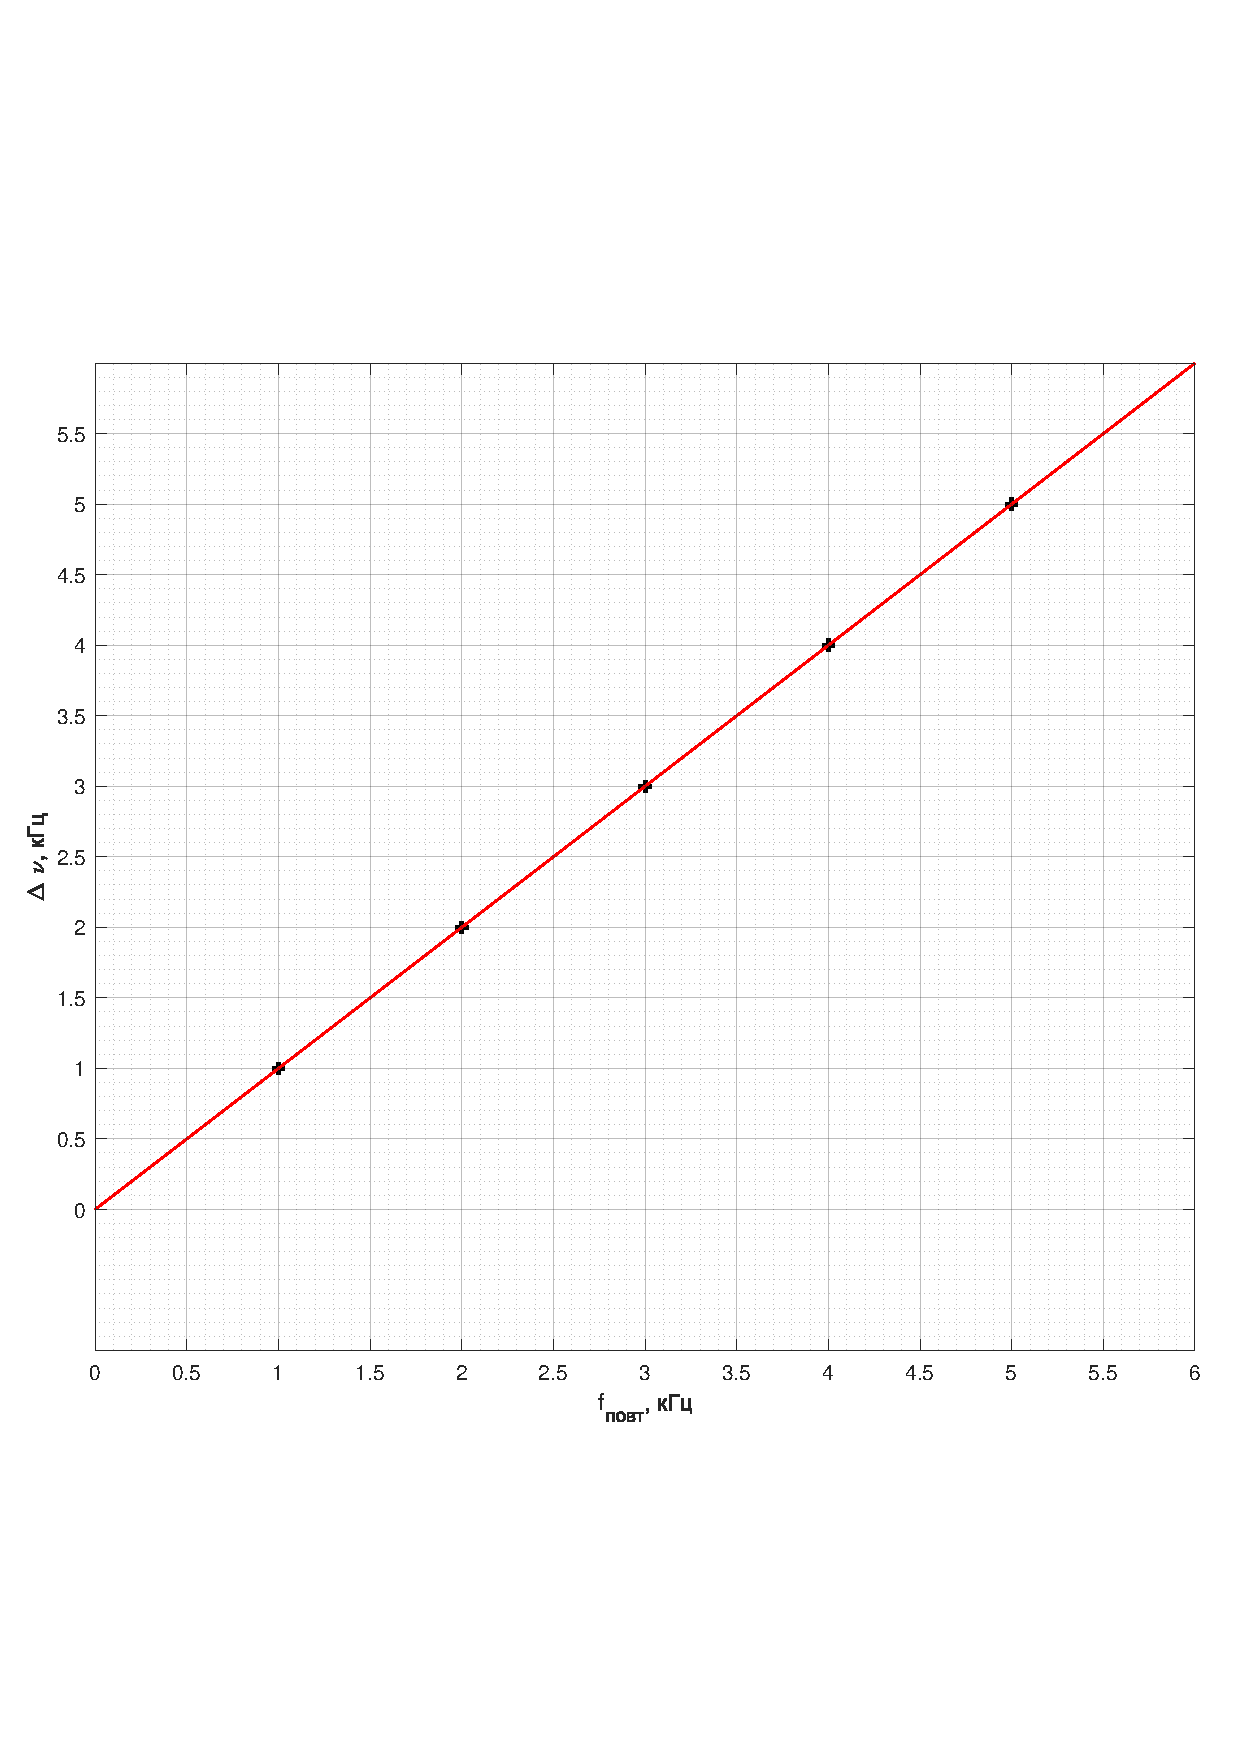
\includegraphics[width=0.7\linewidth]{gr2.pdf} \\
		Рис. 11 -- График зависимости $\Delta \nu(f_{\text{повт}})$
		\label{gr2}
	\end{figure}
\end{center}


\subsection*{Исследование спектра гармонических сигналов, модулированных по амплитуд}


Проведем измерение амплитуды сигнала в зависимости от глубины модуляции, результаты запишем в таблицу \ref{tab7}.

\begin{table}[hbt!]
	\begin{center}
	\begin{tabular}{|c|c|c|c|c|c|c|c|} \hline
		$A(CH1)$, В	&0.2&	0.5&	0.8&	1.1&	1.4&	1.7&	2.0 \\ \hline
		$A_{max}$, дел	&113.7	&130.4	&146.1	&161.9&	176.6&	190.0	&203.0\\ \hline
		$A_{min}$, дел	&92.0	&75.2&	61.5	&46.7&	30.0	&15.3&	0\\ \hline
		$A_{\text{осн}}$, дел	&68.8	&68.8&	68.8&	68.8&	68.8&	68.8&	68.8\\ \hline
		$A_{\text{бок}}$, дел	&3.2	&8.1&	13.1&	18.1&	23.3&	28.2&	33.0\\ \hline
		$m$	&0.105	&0.268	&0.408	&0.552	&0.710&	0.851	&1.000\\ \hline
		$A_{\text{бок}}/A_{\text{осн}}$	&0.047	&0.118	&0.190&	0.263&	0.339	&0.410	&0.480\\ \hline
	\end{tabular}
\caption{Результаты измерений при $f_\text{повт} = 2$ кГц  и $\tau = 100$ мкс}
\label{tab7}
\end{center}
\end{table}

По данным таблицы \ref{tab7} построим график зависимости $A_{\text{бок}}/A_{\text{осн}}(m)$, см. на рис. 12.

\begin{center}
	\begin{figure}[hbt!]
		\centering
		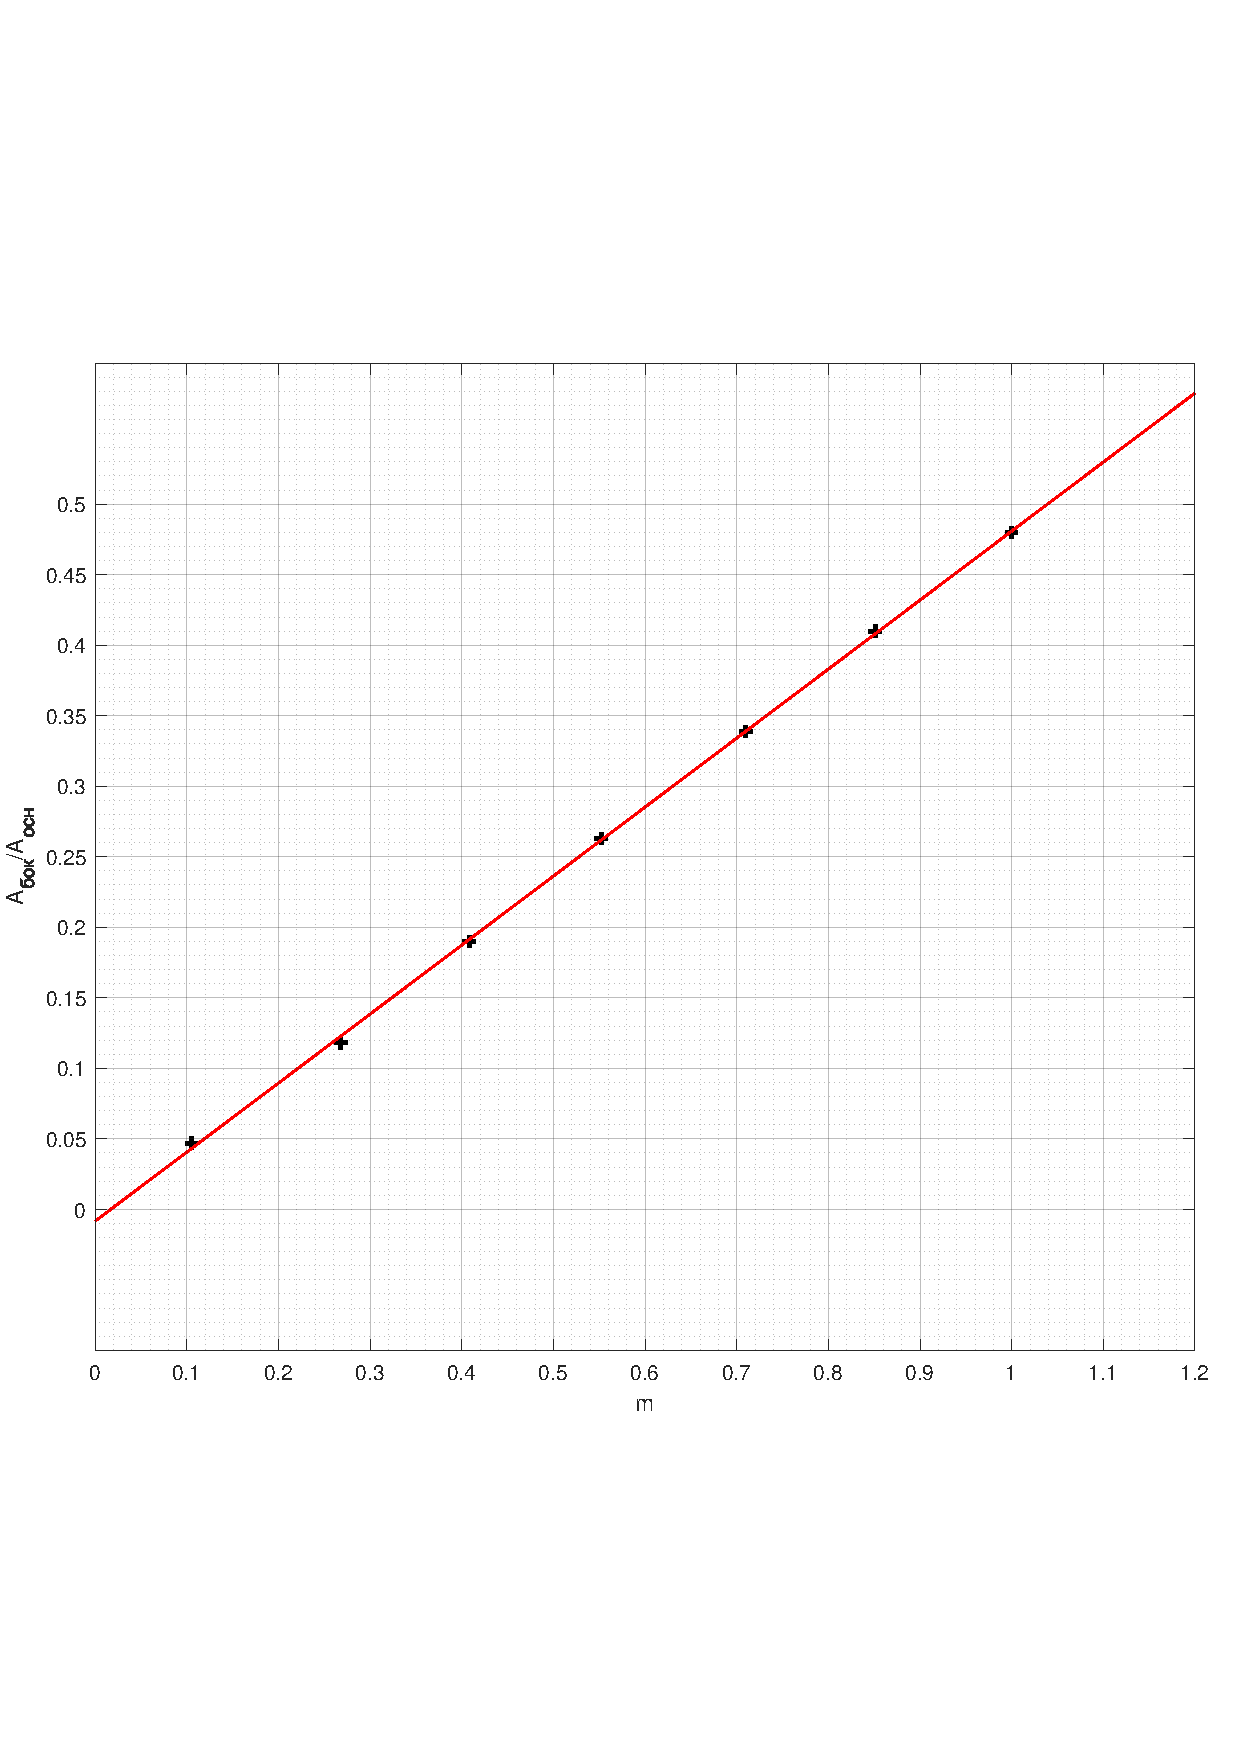
\includegraphics[width=0.72\linewidth]{gr3.pdf} \\
		Рис. 12 -- График зависимости $A_{\text{бок}}/A_{\text{осн}}(m)$
		\label{gr3}
	\end{figure}
\end{center}


Ожидаемы наклон графика $0.5$ совпадает с полученным экспериментально в пределах погрешности: $$k = 0.48 \pm 0.03$$.

При глубине модуляции 100$\%$ посмотрим на изменение спектра при увеличении $f_\text{повт}$, см на рис. 13 -- 14. Видим, что спектр расширяется.

\begin{figure}[!h]
	\parbox[!h]{0.5\textwidth}{\null
		\centering
		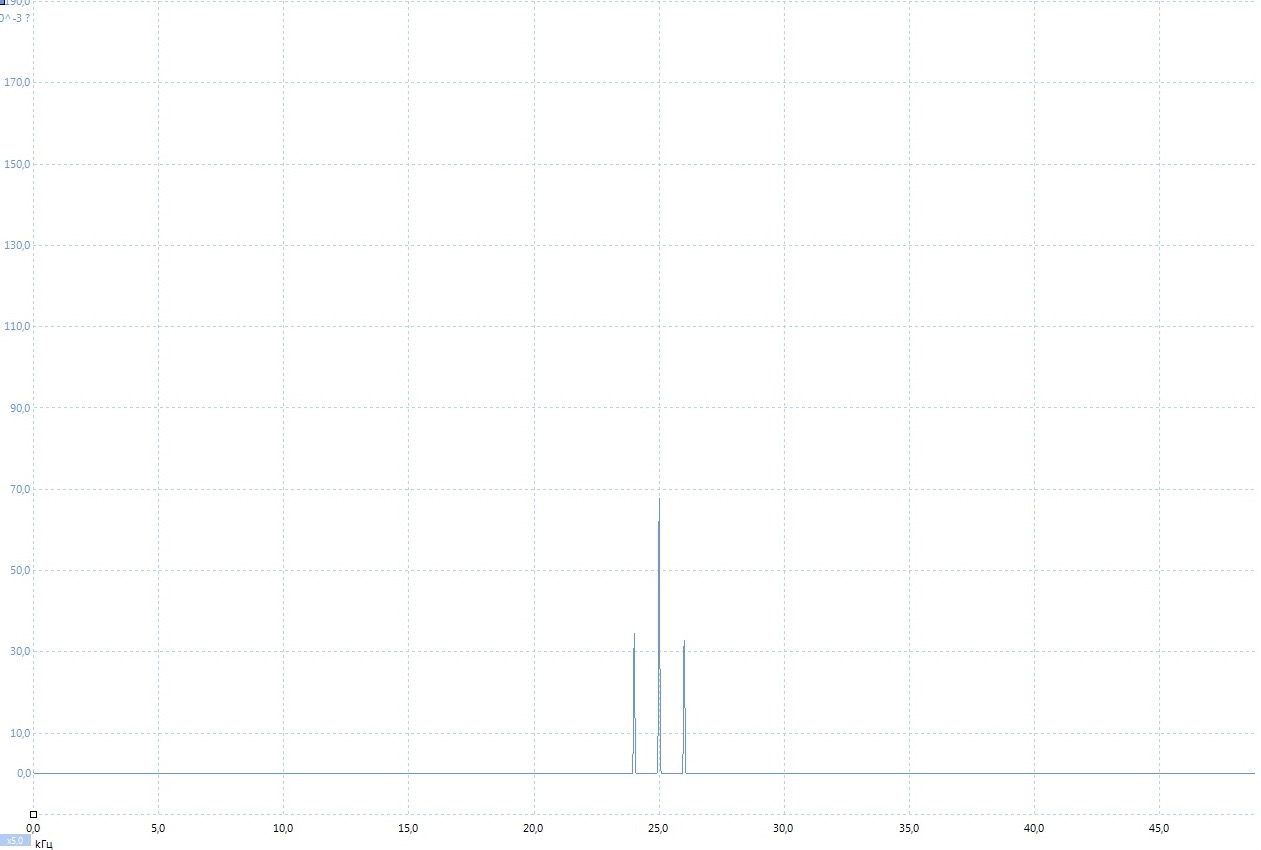
\includegraphics[width = 9cm]{1.jpeg}
		Рис. 13 -- Спектр при $f_{\text{повт}} = 1$ кГц}
	\parbox[!h]{0.5\textwidth}{\null
		\centering
		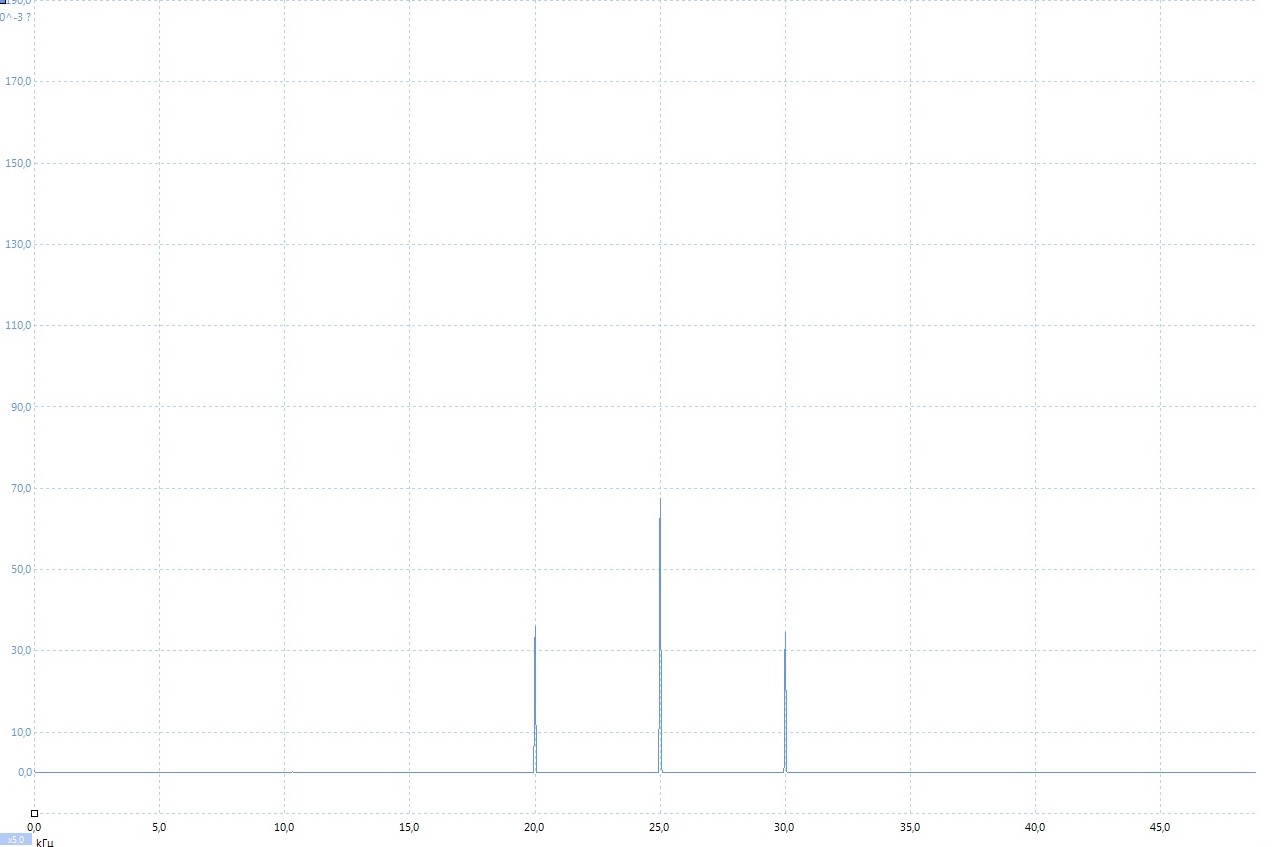
\includegraphics[width = 9cm]{11.jpeg} \\
		Рис. 14 -- Спектр при $f_{\text{повт}} = 5$ кГц}
\end{figure}


\section*{Выводы}
\begin{enumerate}
	\item В ходе лабораторной работы мы изучили спектральный состав периодических электрических сигналов различной формы: последовательности прямоугольных импульсов, последовательности цугов и амплитудно-модулированных гармонических колебаний. 
	\item Проверили выполнение соотношений неопределённости для всех видов сигналов, убедились в его справедливости. 
\end{enumerate}


\end{document}